\documentclass{sig-alternate}

\usepackage{graphicx}

\begin{document}
\title{Social Network based Music Recommendation System}

\numberofauthors{2} 
\author{
\alignauthor
Jiaqi Chen\\
       \affaddr{Stony Brook University}\\
       \email{jiaqichen@cs.stonybrook.edu}\\
      109773151
% 2nd. author
\alignauthor
Jianglin Wu\\
       \affaddr{Stony Brook University}\\
       \email{jianglin.wu@stonybrook.edu}\\
      108075432
}
\maketitle
% ===================    abstract  =====================
\begin{abstract}
Recommendation Systems aim at predicting items or ratings of items that the user are interested in. In this project, we use the dataset from Last.fm, a social music website, to recommend artists to users. Collaborative Filtering (CF) algorithms such as user-based and item-based methods are the dominant techniques. Based on classical CF algorithms, we propose several novel algorithms combining social network information (SocialUserCF) and tag information (TagItemCF) to improve the performance of recommendation. Then, we proposed a hybrid recommendation algorithm (HybridCF) combining with user-based CF, item-based CF. The experiment results show that our novel algorithms have better performance than the classical  algorithms.  We aslo implement tow Bayesian methods and Tag Based TFIDF.  Although the results are not as exciting as CF methods, we learn from the algorithm and try to find the reasons. 
%add bayes
\end{abstract}

\keywords{Recommendation System, Collaborative Filtering, Similarity Measures, Social Network}
% ===================    INTRODUCTION  =====================
\section{INTRODUCTION}
%background
Recommendation systems \cite{rs} have become extremely popular in recent years, and are applied in a variety of areas, such as movies, music, news, books. Actually, a recommender system represents an added value both for consumers, who can easily find products they really like, and for sellers, who can focus their offers and advertising efforts. For music recommendation system,  users can get new artists who suit their personal taste easily with the help of recommendation list rather than searching from millions of possible choices.\\
%classical methods
\indent Collaborative Filtering (CF) is a kind of classical algorithm which is very efficient in practice \cite{amazon}. User-based CF and item-based CF are the two dominant methods. Item-based CF \cite{itembase} is a form of collaborative filtering based on the similarity between items calculated using people's preference of those items, while user-based CF is based on the similarity between users calculated using users' interest. Content-Based recommendation \cite{contentbase, content2} is another popular algorithm which focus on properties of items. Similarity of items is determined by measuring the similarity in their properties. Gori proposed ItemRank \cite{itemrank}, a random-walk based scoring algorithm,  to forecast user preferences by controlling preference flow. However, the speed performance is not ideal when user or item amount is large. 
%add bayes
Bayesian-inference and Naive Bayesian methods construct bayesian network to solve the recommandation problems \cite{bayesianinference}\cite{naivebayesian}.  It seems that few method applies Bayesian to recommandations.  So the results need to be improved.  Our implementations shows this problem.  Last method is Tag Based TFIDF, it's a simple algorithm with TFIDF methodology\cite{tfidf}.  We will find the advantages and disadvantages for each method.  
In addition, as more and more recommendation systems are being used in social network, social network information, such as friendship and followers, can be utilized for recommendation \cite{socialmodel}. And also, Social influences, also called the word-of-mouth effect in the literatures, are known to
be crucial to recommendation system \cite{influence}.
%organications
\indent The rest of the paper is organized as follows. In section 2 we provide a brief description of the dataset. We describe the classical algorithms and our proposed algorithms in section 3. Evaluation criteria is discussed in section 4 and show the results in section 5. Section 6 is the conclusion and future work. Section 7 describes each team member's contribution.
% ===================    Dataset  =====================
\section{Dataset}
This dataset was obtained from Last.fm \cite{lastfm} music website. It contains social networking, tagging, and music artist listening information. The dataset is released in the framework of the 2nd International Workshop on Information Heterogeneity and Fusion in Recommender Systems. Table.1 shows the statistics about the dataset.
For Bayesian-Inference and Naive Bayesian, since we need compute prior and conditional probabilities, we convert numerical user-listened artist data to discrete value.  In out implemtation, we divide user listened number into 5 groups, rating [0,1,2,3,4] for each user and calculate probabilities using discrete rating.  
\begin{table}[!t]
\centering
\caption{Dataset statistics.}
\begin{tabular}{cc}  % {lccc} left-l,right-r,center-c
\\
\hline 
Item  &  Number \\ \hline 
users    &   1892 \\ 
artists    &   17632 \\ 
user-listened artist relations    &   92834 \\ 
bi-directional user friend relations    &   12717 \\ 
tags    &   11946 \\ 
\hline 
\end{tabular}
\end{table}
% ===================    Methods  =====================
\section{Methods}
%  #####  user CF  ##### 
\subsection{User-based Collaborative Filtering}
The main idea of user-based collaborative filtering is to recommend new items of interest for a particular user on the basis of other users' behaviors. Predictions for a user is based on the preference patterns of other people who have similar interests. So at first we find top-k users (\textsl{k} nearest neighbors) who are most similar to the current user, in the music recommendation system, user-user similarity is measured by user's artist preference. The similarity between user \textsl{i} and user \textsl{j} can be calculated as cosine similarity:
\begin{gather*}
sim(i, j)= \frac{\vert N_i  \cap N_j \vert}{\sqrt{\vert N_i \vert \vert N_j \vert}},
\end{gather*}
\indent where $N_i$ is the preference list of user \textsl{i} and $N_j$ is the preference list of user \textsl{j}.\\
\indent Once a \textsl{k} nearest neighborhood of users is formed, system combines the preferences of neighbors to produce a prediction or top-N recommendation for the current user \textsl{u}, the interest of user \textsl{u} to item(artist) \textsl{i} can be expressed as below:
\begin{gather*}
interest(u, i)= \sum_{v \in S(u, K) \cap L_i} sim(u, v),
\end{gather*}
\indent where $S(u, K)$ is the $k$ nearest neighbors of $u$, $L_i$ is the user list who likes item $i$.
%  ##### Social user CF  ##### 
\subsection{User-based Collaborative Filtering using Social Information}
Based User-based Collaborative Filtering, we proposed a new algorithm which uses social Information. Not only users' artist preference but also friendship information is used to measure the similarity between users, therefore, the user-user similarity $sim$ consists two parts: social similarity $sim_a$ and item(artist) preference similarity $sim_b$, the latter is defined in Section 3.1. The social similarity $sim_a$ between user \textsl{i} and user \textsl{j} is described as follow:
\begin{gather*}
sim_a(i, j)= \frac{\vert F_i  \cap F_j \vert}{\sqrt{\vert F_i \vert \vert F_j \vert}},
\end{gather*}
\indent where $F_i$ is the union set of user $i$'s friends list and user $i$ himself, the reason we include user $i$ himself is because if user $a$ and user $b$ are friends, neither $b$ nor $a$ will appear in each other's friends list. So this inclusion would lead to better measurement of social relationships.

The fused similarity $sim$ between user \textsl{i} and user \textsl{j} is defined as follow:
\begin{gather*}
sim(i, j) = a * sim_a(i, j) + (1-a) * sim_b(i, j),
\end{gather*}
\indent where $a$ is the balance parameter for the fusion.
%  ##### item CF  #####
\subsection{Item-based Collaborative Filtering}
Unlike user-based collaborative filtering whose concentration is on the similarity between users, Item-based collaborative filtering focus on the similarity between items. This algorithm assumes that the more common users like two items, the more similar the two items is. Therefore, for the recommendation to current user, at first we get this user's preference list. Then, we find top-k items which are most similar to the items of the preference list. Then use these top-k items as the recommendation list.

The similarity between item \textsl{i} and item \textsl{j} can be calculated as cosine similarity:
\begin{gather*}
sim(i, j)= \frac{\vert U_i  \cap U_j \vert}{\sqrt{\vert U_i \vert \vert U_j \vert}},
\end{gather*}
\indent where $U_i$ is the list of users who like item $i$.
\indent Once a \textsl{k} nearest neighborhood of items are formed, system combines the preferences of neighbors to produce a prediction or top-N recommendation for the current user \textsl{u}, the interest of user \textsl{u} to item(artist) \textsl{i} can be expressed as below:
\begin{gather*}
interest(u, i)= \sum_{i \in S(i, K) \cap L_u} sim(i, j),
\end{gather*}

\indent where $S(i, K)$ is the \textsl{k} nearest neighbors of item $i$, $L_i$ is the item list that user $u$ likes, $sim(i, j)$ is the similarity between item $i$ and item $j$.
%  ##### Tag item CF  ##### 
\subsection{Item-based Collaborative Filtering using Tag Information}
Based Item-based collaborative filtering, we proposed a new algorithm which uses tag Information. From the dataset, we find that each user has tagged several artists, which means each artist have tags as their styles or characteristic. Such property will contribute to the calculation of similarity between artists(items). So we combine the tag information with the classical Item-based collaborative filtering to improve the performance. \\
\indent Therefore, the item-item similarity $sim$ consists two parts: tag similarity $sim_a$ and user preference similarity $sim_b$, the latter is defined in Section 3.3. The tag similarity $sim_a$ between item \textsl{i} and item \textsl{j} is described as follow:
\begin{gather*}
sim_a(i, j)= \frac{\vert T_i  \cap T_j \vert}{\sqrt{\vert T_i \vert \vert T_j \vert}},
\end{gather*}
\indent where $T_i$ is the list of tags of item $i$.

The fused similarity $sim$ between item \textsl{i} and item \textsl{j} is defined as follow:
\begin{gather*}
sim(i, j) = a * sim_a(i, j) + (1-a) * sim_b(i, j),
\end{gather*}
\indent where $a$ is the balance parameter for the fusion.

%  ##### Hybrid CF  ##### 
\subsection{Hybrid Collaborative Filtering}
As we know, item-based and user-based collaborative filtering have different concentration, and both users and items are the two main parts of the real-world recommendation system. Thus, we proposed a hybrid collaborative filtering which take the advantage of Item-based and user-based collaborative filtering. At first we get the top-N recommendation list from both item-based and user-based collaborative filtering. Each list is sorted in ascending order by similarity score and each item has a rank. 
Then go through the two lists and recalculate the rank of items, finally we get the top-N list from the two sorted lists. Below is the equation of recalculation of items' rank:
\begin{gather*}
Rank_i = m * Rank(i, UserCF) + n * Rank(i, ItemCF),
\end{gather*}
\indent where $Rank_i$ is the final rank of item $i$, $Rank(i, UserCF)$ is the $i$'s rank in the result list of user-based CF and $Rank(i, ItemCF)$ is the $i$'s rank in the result list of item-based CF, $m$ and $n$ are the weight parameters.


%  ##### Bayesian-inference  ##### 
\subsection{Bayesian-inference Based Recommendation}
Paper\cite{bayesianinference} introduces a Bayesian-inference based recommendation system for online social network.  A Bayesian network is constructed based on social network for query.  For instance, John is a friend of Amy, Bob, and Casey,.  If John wants to know some artists' rates that he has never listened before,  he sends query to his friends to get the most likely rate to specific artist.  For each of John's friend, for example Amy, we can get John's most probable rating based on historical rating data on common artists between John and Amy.   
\begin{gather*}
R_J | {r_A} = argmax P(R_J=r|r_A).
\end{gather*}
where, $r_A$ is the rating that Amy on this artist. 
Similarly, after we get all the rating from John's friends,  the estimate rate for specify artist is:
\begin{gather*}
R_J | {\{r_A,r_B,r_C\}} = argmax P(R_J=r|r_A,r_B,r_C).
\end{gather*}
Unfortunately, in practice, it's hard to estimate the joint conditional distribution between John and all his friends.  So, the Bayesian network is built to simplify the problem.  Set John as the root, all of his friend is his child node  in the Bayesian network.  And we assume that each friend's rating is independent to each other.  Finally, we can calculate that:
\begin{gather*}
R_J | {\{r_A,r_B,r_C\}} = \frac{P(r_A,r_B,r_C|r_J)P(r_J)} {\sum_{r} P(r_A,r_B,r_C|R_J=r)P(R_J=r)} 
\end{gather*}
\begin{gather*}
\indent  \indent \indent \indent \indent \indent=\frac{P(r_A|r_J)P(r_B|r_J)P(r_C|r_J)P(r_J)} {\sum_{r} P(r_A,r_B,r_C|R_J=r)P(R_J=r)} .
\end{gather*}
However, the problem is that, John's friend may not have rating on the artist that John queries.  We will recurssively query on John's friend' friends.  In the implementation, we set the hop (recurssive depth) to 1, which means we query up to user's friend's friend.  If it's still empty, we just ignore that factor.  

%  ##### Naive Bayes  ##### 
\subsection{Naive Bayesian Method}
Paper\cite{naivebayesian} improves Naive Bayesian method to handle the situation where each factor has more influence. Author adjusts the original Naive Bayesian to 
\begin{gather*}
p(m_x|m_{u_1},m_{u_2},...)=p(m_x)q^\frac{c_n}{n}.
\end{gather*}
where
\begin{gather*}
q=\frac{p(m_{u_1},m_{u_2},...|m_x)}{p(m_{u_1},m_{u_2},...)}=\frac{p(m_{u_1}|m_x)}{p(m_{u_1})} \frac{p(m_{u_2}|m_x)}{p(m_{u_2})} ....
\end{gather*}
and $m_x$ is the probability that user likes this specific artist, $m_{u_i}$ is the prior probability calculated from trainining data, $n$ is the number of known artists for current user, $c_n$ is calculated by experiments, based on author's conclusion, $c_n$ is 3 for most cases.  In the implementation, we convert rate to two parts: if rating is greater than threshold rating, then user likes it, otherwise,  doesn't like.  The result indicates the confidence of a user's interests to the artist.


%  ##### Tag Based TF-IDF ##### 
\subsection{Tag Based TF-IDF}
We learn another recomandation method from a book called Tag Based TF-IDF recommandation.  The basic idea is simple.  1. count most common tags for each user. 2. for each tag, find the artist who has the highest counts with this tag.  3. For each user, find tags from step 1 and recommand artist from step 2.  It can be described as follow: 
\begin{gather*}
p(u,i)=\sum_{b} \frac{n_{u,b}}{log(1+n_b^{(u)})}\frac{n_{b,i}}{log(1+n_i^{(u)})}.
\end{gather*}
where $B(u)$ is the tag set for user u, $B(i)$ is the tag set for artist i, $n_{u,b}$  is the count of tag b that user u marks, $n_{b,i}$ is the count of tag b that artist i is marked, $n_b^{(u)}$ is the count of distinct user who has used tab b and $n_i^{(u)}$ is the count of distinct user who has tagged on artist i. 


% ===================    Evaluation  =====================
\section{Evaluation Criteria}
In this section we briefly review basic evaluation criteria (precision, recall, coverage) for recommendation system. A good recommendation algorithm is expected to be of high precision,  recall and coverage. Here we define some notation:
\begin{itemize}
\item $R_u$: recommendation list for user $u$.
\item $T_u$: actual preference list of user $u$ from testing set.
\item $I$: item set from testing set.
\end{itemize}
%------
\subsection{Precision}
Precision is the most important evaluation criteria for recommendation system, which describes the accuracy performance. Precision is the ratio of correct recommendation items to the whole recommendation set.
It is defined as follow:
\begin{gather*}
Precision = \frac{\sum_{u} {\vert   R_u  \cap T_u   \vert}}   {  \sum_{u} \vert  R_u   \vert }.
\end{gather*}
%------
\subsection{Recall}
Recall is the another important evaluation criteria which is the proportion of correct recommendation items to the preference set of all users.
It is defined as follow:
\begin{gather*}
Recall = \frac{\sum_{u} {\vert   R_u  \cap T_u   \vert}}   {  \sum_{u} \vert  T_u   \vert }.
\end{gather*}
\subsection{Coverage}
Coverage is the ratio of recommendation items to the item set which measures the percentage of items that an algorithm is able to recommend.
Low coverage indicates that the algorithm can access and recommend only a small number
of distinct items (usually the most popular ones) which often results in little diverse recommendations. From this viewpoint, coverage can be also considered as a diversity metric.
Coverage is defined as follow:
\begin{gather*}
Coverage = \frac{{\vert    \cup R_u    \vert}}   { \vert  I   \vert }.
\end{gather*}
% ===================    Results  =====================
\section{Experiment Results}
In order to test our algorithms, we randomly sample 80\% of the dataset as training set and the rest 20\% as the testing set. We test the total 8 algorithms, including classical ones and the novel methods proposed by us. Fig.1 shows the precision of the 8 algorithms, Fig.2 shows the recall and coverage is shown as Fig.3.

\begin{figure}[h]
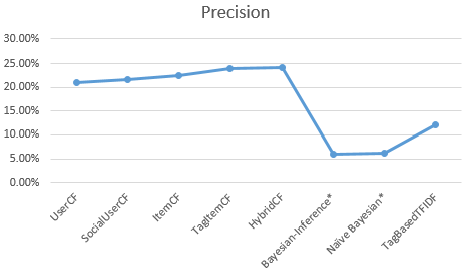
\includegraphics[width=\linewidth]{image/Precision}
\begin{center}
Fig.1
\end{center}
\end{figure}

\begin{figure}[h]
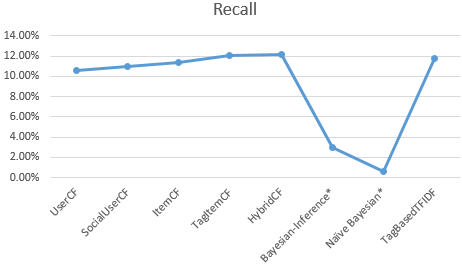
\includegraphics[width=\linewidth]{image/Recall}
\begin{center}
Fig.2
\end{center}
\end{figure}

\begin{figure}[h]
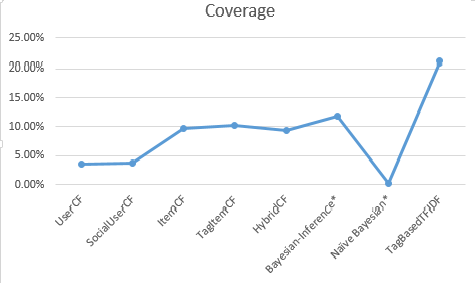
\includegraphics[width=\linewidth]{image/Coverage}
\begin{center}
Fig.3
\end{center}
\end{figure}


* Bayesian-Inference Based Recommandation and Naive Bayesian generate low Precision and Recall for all the test user.  Therefore, we set threshold to eliminate those test user with obvious wrong recommand items.  

From Fig.1 we know that UserCF, SocialUserCF, ItemCF tagItemCF and HybridCF have about 20\% to 25\% precision.  And by improving algorithms, we see that ItemCF and tagItemCF have better Precision, Recall and Coverage than UserCF and SocialUserCF. The HybridCF, which combies all the advantages of those four CFs, has the best outcomes.  However, Bayesian-Inference and Naive Bayesian only have about 6\% precision.  The reason may be as follows:  Bayseian-Inference needs query friends' rating for each user, from the program we get that there are 17213 queries return no rating (which means the probability of having any rate is low, in our implmentation, we set threshold to 0.1),  442537114 of the queries return estimate rating, which is about 99.76\% of all queries. The actual rate, which reads from training data is only about 0.24\%.  So, each time when user queries about a artist from his friend,  most of the return rating is estimated.  We tried different rate and probability threshold (drop whose queries with any rating probabilities smaller than the threshold ), the result doesn't improve the Precision. Meanwhile Recall drops as rate and probability threshold increase.  From Fig. 3, we can find that even though the Precision and Recall for Bayesian-Inference is not satisfactory, its Coverage is higher than other CF methond.  It does recommand different artists for differenct users based on their social network.  Tag Based TFIDF performs the best coverage and Naive Bayesian needs to be modified to improve its result.








% ===================    CONCLUSION  =====================
\section{CONCLUSION AND FUTURE WORK}
%add bayes
There are a lot challenges for recommendation system, such as data sparsity, scalability and cold start. Data sparsity may cause low or none overlap between two users, which would lead to low precision of the recommendation algorithms. Singular Value Decomposition (SVD) \cite{svd} is a efficient way to solve the problem of data sparsity.
As the data is growing very fast, it is therefore essential to consider the computational cost issues. Hadoop or other distributed systems are used to handle big data for recommendation \cite{hadoop}.
Cold start happens when new users enter the system, there is usually not enough information to do the recommendation. \cite{cold} introduced a efficient solution for cold start.
Therefore, for better performance, we should figure out these challenges and utilize more helpful information from the dataset.

The paper of Bayesian-inference Based Recommendation use Mean Absolute Error to test the performance.  Their result also shows that the perfermance of the Bayesian-inference is worse than CF, however, the coverage is better in some cases.   And the data they use contains about one million ratings for 3952 movies and 6040 users.  Compare to our data set, we only have about 0.1 million ratings for 17632 artists and 1892 users.    Same for the Naive Bayesian method, data set in the paper has 7 million records of 714 items from 375195 users, which has more prior probability information. We think that our number of rating data is not engouth to set up the Bayesian network.   Naive Bayesian is the worst among all the methods, since it doesn't include social realtionship or tag information.  



%===================   CONTRIBUTIONS ====================
\section{Contributions}
\begin{itemize}
\item Jiaqi Chen is responsible for data collection and clean, algorithms design and implementation, including UserCF, SocialUserCF, ItemCF, TagItemCF and HybridCF.
\item Jangling Wu is responsible for data division, evaluation criteria design, algorithms design and 
implementation, including Bayesian-inference Based Recommendation, Naive Bayesian CF and Tag Based TF-IDF.
\end{itemize}

\bibliographystyle{unsrt}
\bibliography{bibliography}
\end{document}
